\section{Overview of \FW{}}\label{sect:Overview}
In this section, we give an overview of \FW{} and its major components. The sections following this go into detail about some of the individual parts of the framework. \FW{} can be downloaded at the  Git repository at the following url: \url{https://github.com/Betaboxguugi/SkiRaff}

The purpose of \FW{} is to assist in functional source-to-target testing of ETL programs developed using pygrametl. As such, testing is performed by asserting about properties of DWs, which have been populated by a pygrametl program. The focus of testing lies on data loss and business rules. Testers can make assertions about new functionality or perform regression testing using old assertions. Testing is performed at the system level. Thus, the extraction, transformation and loading components are integrated prior to test. The framework is not designed for exhaustive testing. It is instead meant to assist in reaching an adequate level of test coverage.

\FW{} contains four major components:
\begin{itemize}
\item DWPopulator
\item DWRepresentation
\item Predicates
\item Case 
\end{itemize}

The purpose of the DWPopulator is to execute the pygrametl program under test and populate the corresponding DW. When the DW is populated, we can run tests on it.  Testers may choose, how the program is executed. They may just run it as usual, using the connections to sources and DW hardcoded into the program. However, these data sources may contain actual data collected and used by an organization. Because of regulations, such data may not be available for testers to use. Instead, \FW{} allows testers to dynamically insert test sources and DW into the program before execution. This way, test data may easily be switched in and out without messing with the program itself.  

After executing the program, the DWPopulator builds a DWRepresentation object corresponding to the populated DW. DWRepresentation is a class made to contain structural information about a DW. It also allows for easy access of the DW tables and their metadata.

The Predicates are a family of classes used to make assertions about the properties of a populated DW. All of them inherit from the Predicate class. Testers assert by instantiating a predicate class with the tables of interest, along with some additional arguments depending on the predicate type. Once instantiated, a predicate can be executed to check, whether the defined assertion holds or not. After execution, it creates a Report object that indicates the result of the check.

Case is a class representing a test case. It serves as the tester’s primary way of interacting with \FW{}. The class is rather simple, executing a set of predicates on a DW through a DWRepresentation. After a predicate is executed, Case displays the contents of the Report object made by the predicate to the user.  Note that since Case takes a DWRepresentation as input, the user does not have to run DWPopulator to perform testing. Testers may construct a DWRepresentation themselves.

\subsection{Example Scenario}

\begin{figure}
\centering
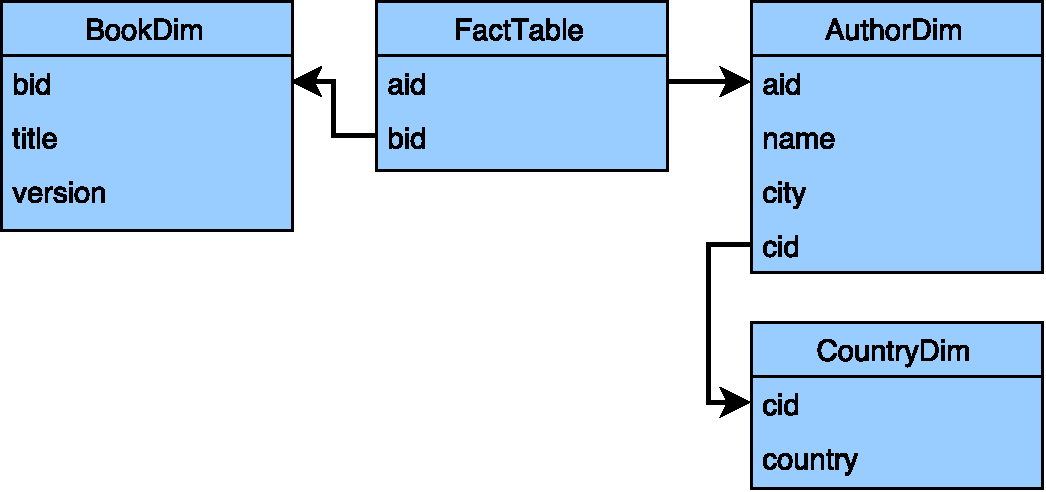
\includegraphics[width=0.48\textwidth]{figures/example_dw.pdf}
\caption{BookAndAuthor DW schema}
\label{fig:exdw}
\end{figure}

This subsection will be used to describe an example scenario, in which \FW{} is used to conduct tests. For this example, we imagine that we have already written a pygrametl program. This pygrametl program performs the necessary ETL operations to populate the BookAndAuthor test DW using two databases as sources. All three are constructed with SQLite, using the python module sqlite3, which upholds the PEP 249 standard. But any other module supporting PEP 249 could have been used. The DW schema of BookAndAuthor can be seen in \Cref{fig:exdw}. E.g. we wish to test that our program correctly populates the DW, so that the fact table has exactly 99 rows. We also assert that there is referential integrity. This test is performed through the python script in \Cref{Case.py}. We explain the code below, with an in-depth description of each module used in later sections.

\insertcodefile{Case.py}{Example of a \FW{} program}

\begin{description}
\item[line 3-15] As we are using both test sources and a test DW, we wish to have these used as replacements for the data connections, which are hardcoded into the pygrametl program. This requires that the tester first creates PEP 249 connections to the sources. We then instantiate the DWPopulator with some parameters. These describe the program to run, how to connect to the test DW as well as the replacement sources.  After instantiation, we execute the object by calling the \texttt{run} method. This runs the pygrametl program with the test sources and DW. It then returns a DWRepresentation object corresponding to the BookAndAuthor test DW.

\item[line 16-20] We instantiate two Predicate objects. One asserts that  the fact table has exactly 99 rows. The other asserts that there is referential integrity in the DW.

\item[line 21-25] We instantiate a Case with our DWRepresentation and Predicate objects. We then call its \texttt{run} method. This runs each predicate on the populated BookAndAuthor DW. When each predicate has been executed, their results are reported to the tester.   
\end{description}

In the following sections, we go into detail about the implementation of the three major components of \FW{}, as discussed in this section. These include DWPopulator, DWRepresentation as well as all of the Predicate classes. Case will not be covered as its implementation is trivial.
